%%% paper.tex — Structural Health Monitoring for Governed Human-Agent Systems
%%% ACM sigconf format (nonacm to suppress copyright blocks)
\PassOptionsToPackage{table}{xcolor}
\documentclass[sigconf,nonacm]{acmart}

%% Packages
\usepackage{tikz}
\usetikzlibrary{shapes.geometric, arrows.meta, positioning, calc, patterns, decorations.markings, fit}
\usepackage{pgfplots}
\pgfplotsset{compat=1.18}
\usepackage{booktabs}
\usepackage{amsmath}
\usepackage{enumitem}

%% Remove ACM reference format line
\settopmatter{printacmref=false}
\renewcommand\footnotetextcopyrightpermission[1]{}
\pagestyle{plain}

%% Colors
\definecolor{bandgreen}{RGB}{200,230,200}
\definecolor{bandred}{RGB}{240,200,200}
\definecolor{bandamber}{RGB}{250,230,180}
\definecolor{vtgreen}{RGB}{76,175,80}
\definecolor{vtyellow}{RGB}{255,193,7}
\definecolor{vtred}{RGB}{244,67,54}
\definecolor{cellgreen}{RGB}{200,240,200}
\definecolor{cellred}{RGB}{255,200,200}
\definecolor{cellamber}{RGB}{255,240,200}
\definecolor{coordblue}{RGB}{33,100,205}
\definecolor{gatedorange}{RGB}{230,120,20}
\definecolor{flowblue}{RGB}{66,133,244}
\definecolor{flowgray}{RGB}{220,220,220}

\begin{document}

\title{Structural Health Monitoring for Governed Human-Agent Systems:\\A Homeostatic Approach}

\author{Carlos R. B. Azevedo}
\affiliation{%
  \institution{Independent Researcher}
  \country{United Kingdom}
}
\email{carlos@crbazevedo.com}

\begin{abstract}
Multi-agent AI systems require governance: rules that determine how much
autonomy each agent has. Current approaches enforce governance through
static policies (risk tiers, approval workflows) or runtime policy engines.
These tell you whether a specific action is permitted. They do not tell you
whether your governance \emph{configuration} is healthy.

We present a formal model for \textbf{governance health monitoring} --- a
structural diagnostic that auto-encodes governance events into an
expression tree, computes two health metrics (coordination health and
gatedness), and classifies the governance configuration as stable,
oscillating, or drifting. We prove five formal properties: the regulatory
actions always improve their target metric, they don't interfere with each
other, the evaluation always terminates, and the application order doesn't
matter.

We evaluate on four governance scenarios from a real multi-agent system
(CARLOS-OS). The well-governed configuration converges. The ungoverned
configuration drifts. The non-obvious finding: the \emph{over-governed}
configuration --- 100\% review rate, all high-tier risk gates --- enters a
limit cycle. It is structurally unstable because nothing passes.
A threshold-based classifier labels this ``perfectly governed.'' Our
structural diagnostic catches it.

The model, interpreter (128 tests), and live demonstration are open source
at \url{https://github.com/crbazevedo/seam}.
\end{abstract}

\begin{CCSXML}
<ccs2012>
<concept>
<concept_id>10011007.10011074.10011099</concept_id>
<concept_desc>Software and its engineering~Software verification and validation</concept_desc>
<concept_significance>500</concept_significance>
</concept>
<concept>
<concept_id>10011007.10011074.10011111</concept_id>
<concept_desc>Software and its engineering~Software evolution</concept_desc>
<concept_significance>300</concept_significance>
</concept>
</ccs2012>
\end{CCSXML}

\ccsdesc[500]{Software and its engineering~Software verification and validation}
\ccsdesc[300]{Software and its engineering~Software evolution}

\keywords{governance, multi-agent systems, self-adaptive systems, homeostasis, structural health monitoring, runtime verification}

\maketitle

%% ============================================================
%% SECTION 1: INTRODUCTION
%% ============================================================
\section{Introduction}

\subsection{The Problem}

Consider a team of AI agents working alongside a human operator. Some
actions are safe to automate (reading files, running tests). Others are
risky (sending emails to board members, deploying to production). A
governance framework assigns risk tiers --- the higher the tier, the more
human oversight is required.

This pattern is widespread. The EU AI Act~\cite{euaiact} defines four risk
levels. NIST's AI Risk Management Framework~\cite{nist} prescribes
governance functions. Microsoft's Agent Governance Toolkit~\cite{microsoft}
enforces policies at runtime. In practice, most multi-agent systems use
some form of tiered governance: AutoGen's conversation
patterns~\cite{autogen}, CrewAI's role-based delegation, LangGraph's state
machine guards.

The governance \emph{enforcement} problem is largely solved: given a
policy, check whether each action complies. But a different question is
unanswered:

\begin{quote}
\textbf{Is the governance configuration itself healthy?}
\end{quote}

A system where every action is gated at the highest tier has 100\%
compliance. It is also paralyzed --- nothing gets done without approval.
A system where every action is autonomous has 0\% overhead. It is also
uncontrolled. Both are valid governance configurations. Neither is healthy.

\subsection{Why Governance is Homeostatic}

Healthy governance occupies a band between two failure modes:

\begin{itemize}[leftmargin=*]
  \item \textbf{Under-governed} (too open): actions pass without oversight.
    Risk increases. Trust erodes after incidents.
  \item \textbf{Over-governed} (too closed): every action requires approval.
    Throughput drops. Teams route around the governance to get work done,
    creating shadow processes that are \emph{less} governed than the original.
\end{itemize}

This is not a problem with a fixed solution. The right governance level
changes with conditions --- deadline pressure, team trust, incident history.
Governance is \emph{homeostatic}: it must stay within a band, and that band
is maintained through continuous adjustment, not static rules.

\subsection{Contributions}

We present a formal model where:

\begin{enumerate}[leftmargin=*]
  \item \textbf{Governance events} (agent handoffs, risk-tier assignments,
    approval decisions, governance checks) are auto-encoded into an
    \textbf{expression tree} --- a structural representation of the
    governance state. (Section~\ref{sec:model})

  \item Two \textbf{health metrics} are computed from the tree:
    \emph{coordination health} (how well agents are coordinating) and
    \emph{gatedness} (how much is being gated vs.\ passing freely).
    (Section~\ref{sec:model})

  \item A \textbf{homeostatic evaluator} detects when either metric exits a
    health band and prescribes specific interventions: ``add coordination''
    or ``tighten gates.'' We prove five formal properties guaranteeing
    predictable evaluator behavior. (Section~\ref{sec:formal})

  \item Evaluation on four governance scenarios from a real system shows the
    model correctly distinguishes stable, drifting, and oscillating
    governance --- including the non-obvious over-governance failure mode.
    (Section~\ref{sec:eval})
\end{enumerate}

%% ============================================================
%% SECTION 2: BACKGROUND AND RELATED WORK
%% ============================================================
\section{Background and Related Work}

\subsection{Governance in Multi-Agent AI Systems}

The shift from single-agent to multi-agent AI systems has created a
governance gap. Bose~\cite{bose} presents the first systematic survey of
governance frameworks for LLM agent collectives, identifying three
failure modes --- operational miscoordination, strategic misalignment,
adversarial collusion --- and taxonomizing five governance models
(hierarchical, prescriptive, democratic, economic, emergent). The
survey finds industry favors deterministic but brittle models while
academia explores adaptive but chaotic ones.

Microsoft's Agent Governance Toolkit~\cite{microsoft}, released April
2026, provides runtime policy enforcement: zero-trust identity, execution
sandboxing, compliance grading, and circuit breakers, covering all 10
OWASP agentic AI risks with sub-millisecond enforcement. It addresses
\emph{per-action enforcement} but not \emph{configuration-level health}.
Our approach is complementary: structural health monitoring answers ``is
the governance working?'' alongside policy engines that answer ``is this
action permitted?''

Li et al.~\cite{liarch} propose a layered governance architecture
(sandboxing, intent verification, zero-trust authorization, audit
logging). Xiang et al.~\cite{agentguard} introduce AgentGuard for
runtime verification with probabilistic model checking. These provide
external verification and enforcement. Our model makes governance health
an intrinsic structural property.

\subsection{Adjustable Autonomy and Trust}

The question ``how much autonomy should each agent have?'' has been
studied extensively. Parasuraman et al.~\cite{parasuraman} define 10
Levels of Automation. Kaber~\cite{kaber} reviews how LoA taxonomies have
been used and critiques their limitations for increasingly autonomous
systems. SARI~\cite{sari} formulates shared autonomy as a POMDP, learning
assistance across repeated interactions.

On the trust side, Lee and See~\cite{leesee} define trust as attitude
under uncertainty, distinguishing analytic, analogical, and affective
processes. Hoff and Bashir~\cite{hoffbashir} integrate empirical evidence
into a three-layered model (dispositional, situational, learned). Kim et
al.~\cite{kim} find that user involvement in LLM planning \emph{fails}
to calibrate trust --- plausible plans mislead users --- arguing that
governance must be structural, not reliant on user judgment of agent plans.

These approaches model autonomy and trust for \emph{single} agent-human
pairs. We extend to multi-agent systems where the health question is
about the \emph{configuration} --- the distribution of autonomy levels
and coordination patterns across a team.

\subsection{Self-Adaptive Systems}

The MAPE-K reference architecture~\cite{mapek} (Monitor-Analyze-Plan-Execute
over Knowledge) is the standard model for self-adaptive software. Our
evaluator follows the MAPE-K pattern: Monitor (compute metrics), Analyze
(detect deviations from health band), Plan (select regulatory action),
Execute (prescribe intervention), Knowledge (expression tree).

The key difference: MAPE-K loops operate on \emph{numerical} state
variables. Our monitor operates on \emph{structural} state --- an
expression tree whose topology encodes the governance configuration.
Metrics emerge from the structure itself, not from externally defined
sensor readings.

Weyns~\cite{weyns} provides a comprehensive introduction to self-adaptive
systems engineering. Sanwouo et al.~\cite{aware} propose AWARE as a
successor to MAPE-K, distributing the feedback loop and making it
goal-driven. Li et al.~\cite{ligen} map how generative AI can enhance
each MAPE-K phase. Our contribution provides a formal structural substrate
for the Monitor and Analyze components --- one where governance health has
algebraic properties.

\subsection{Organizational Cybernetics}

Ashby's Law of Requisite Variety~\cite{ashby} states that a controller
must have at least as much variety as the system being controlled. Beer's
Viable System Model~\cite{beer} applies this to organizations, modeling
five subsystems that maintain viability through homeostatic loops. Perez
Rios~\cite{perezrios} recently applied Beer's VSM to AI governance,
mapping organizational pathologies to AI failure modes.

Our model operationalizes the cybernetic principle: the health band IS the
homeostatic target, the regulatory actions (BIND, VEIL) ARE the requisite
variety, and the convergence/divergence/limit-cycle classification IS the
viability diagnosis.

\subsection{Formal Runtime Monitoring}

Runtime verification~\cite{leucker} checks whether a system execution
satisfies a formal property. Tools like Uppaal and PRISM verify
temporal-logic specifications. These approaches answer ``does the trace
satisfy $\varphi$?'' --- a binary yes/no. Our approach answers ``is the
governance configuration in a healthy structural state?'' --- a continuous
diagnostic with specific remedies.

%% ============================================================
%% SECTION 3: THE GOVERNANCE HEALTH MODEL
%% ============================================================
\section{The Governance Health Model}\label{sec:model}

\subsection{Governance Events}

We model governance as a stream of typed events. Table~\ref{tab:events}
shows the event types and their encodings.

\begin{table}[t]
  \caption{Governance Event Encoding}\label{tab:events}
  \small
  \begin{tabular}{@{}lll@{}}
    \toprule
    \textbf{Event Type} & \textbf{Operation} & \textbf{Effect} \\
    \midrule
    Coordination & Agent A $\to$ Agent B & Coordination binding \\
    Gated action & VT$k$ action & Gate with threshold $\theta_k$ \\
    Governance check & Preflight check & Holding gate \\
    Observation & File ingestion & Witness link \\
    Resolution & Human approval & Gate: passing $\to$ holding \\
    \bottomrule
  \end{tabular}
\end{table}

\subsection{The Governance Structure}

Each event modifies an expression tree --- the \textbf{governance structure}.
The tree is built from three node types:

\paragraph{Coordination binding ($a \cdot b$).}
Represents bilateral coordination between two parties. When Agent~A hands
off work to Agent~B, a binding is created. Bindings are symmetric
($a \cdot b = b \cdot a$), associative ($(a \cdot b) \cdot c = a \cdot
(b \cdot c)$), and grounded in an empty element ($a \cdot \varnothing = a$).
This gives them the algebraic structure of a commutative monoid --- the
simplest structure that captures ``coordination without ordering.''

\paragraph{Gate ($a\;|\theta|\;b$).}
Represents a governance boundary with autonomy level~$\theta$. When the
system's \emph{reach} (a parameter representing the current operating
context) exceeds $\theta$, the gate passes and the content is visible.
When reach is below~$\theta$, the gate holds and the content is
\emph{veiled} --- it has structural weight but is not directly accessible.

The mapping from risk tiers to gate thresholds is shown in
Table~\ref{tab:risktiers}.

\begin{table}[t]
  \caption{Risk Tier to Gate Threshold Mapping}\label{tab:risktiers}
  \small
  \begin{tabular}{@{}llcl@{}}
    \toprule
    \textbf{Risk Tier} & \textbf{Description} & $\boldsymbol{\theta}$ & \textbf{Behavior (reach=0.5)} \\
    \midrule
    VT0 & Full autonomy & 0.1 & Always passes \\
    VT1 & Act and notify & 0.3 & Passes \\
    VT2 & Needs approval & 0.5 & Marginal \\
    VT3 & Propose and wait & 0.7 & Holds \\
    VT4 & Stop and escalate & 0.95 & Always holds \\
    \bottomrule
  \end{tabular}
\end{table}

\paragraph{Adaptive gate ($a\;|\mathrm{breath}(b,a,f)|\;b$).}
A gate whose threshold oscillates over time:
$\theta_{\mathrm{eff}} = \theta_{\mathrm{base}} + A \sin(c \cdot f)$,
where $A$ is amplitude, $c$ is the current cycle, and $f$ is frequency.
This models Action Opportunity Windows (AOWs) --- time-bounded intervals
during which governance gates open.

\paragraph{Evaluation iteration ($\mu\, x.\, \mathrm{body}$).}
The governance cycle. Each iteration substitutes the previous governance
state into the body, evaluates it, measures the resulting structure,
applies regulation if needed, and checks for stability.

\subsection{Health Metrics}

Two metrics are computed from the governance structure by a single tree walk:

\paragraph{Coordination health.}
\begin{equation}\label{eq:coordination}
  \mathrm{coordination} = \frac{\text{binding\_nodes}}{\max(\text{total\_nodes} - 1,\; 1)}
\end{equation}
Measures how much of the governance structure consists of bilateral
coordination. Range: $[0, 1]$. High coordination health means agents are
working together; low means agents are isolated.

\paragraph{Gatedness.}
\begin{equation}\label{eq:gatedness}
  \mathrm{gatedness} = \frac{\text{gates\_passing}}{\max(\text{total\_gates},\; 1)}
\end{equation}
Measures what fraction of governance gates are currently passing. Range:
$[0, 1]$. Neutral (0.5) if no gates exist. High gatedness means most
actions pass without oversight; low means most are held for review.

\subsection{The Health Band}

Healthy governance occupies a band (Figure~\ref{fig:healthband}):

\begin{itemize}[leftmargin=*]
  \item \textbf{Coordination:} $[0.3,\; 0.7]$ --- agents are coordinating
    but not over-coupled.
  \item \textbf{Gatedness:} $[0.2,\; 0.6]$ --- some actions pass freely,
    some are gated.
\end{itemize}

When either metric exits the band, the evaluator fires a regulatory action:

\textbf{BIND} (coordination too low): ``Agents are too isolated. Add
cross-agent review, require handoffs, increase coordination.''

\textbf{VEIL} (gatedness too high): ``Too much is passing without
oversight. Tighten the risk tier for recent action types, add governance
gates.''

%% --- FIGURE 1: Health Band ---
\begin{figure*}[t]
  \centering
  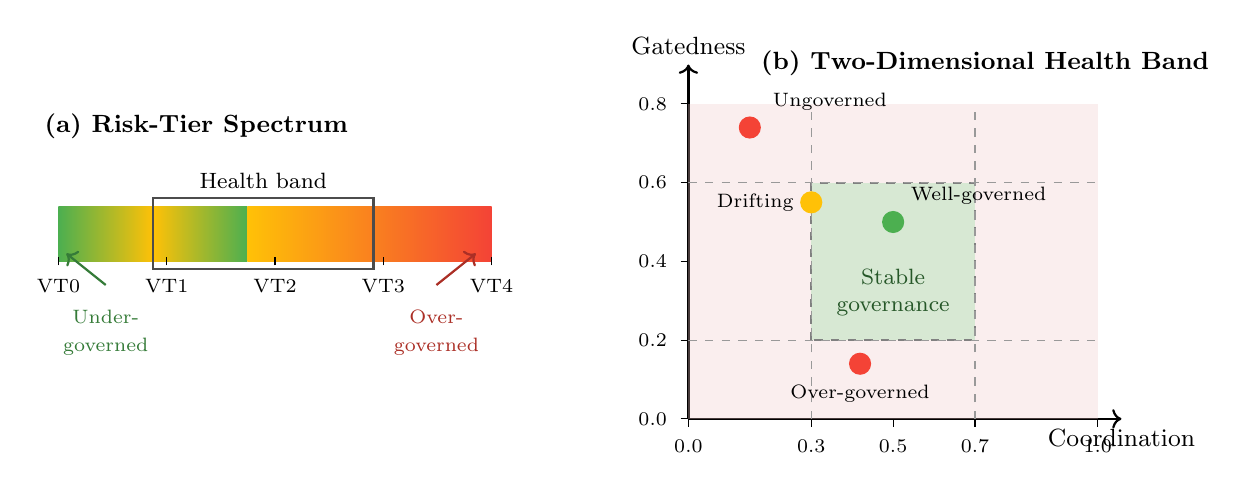
\begin{tikzpicture}
    %% LEFT PANEL: Risk-tier spectrum
    \begin{scope}[xshift=0cm]
      \node[anchor=north west, font=\small\bfseries] at (-0.3,4.0) {(a) Risk-Tier Spectrum};

      %% Gradient bar
      \shade[left color=vtgreen, right color=vtgreen, middle color=vtyellow]
        (0,2) rectangle (2.4,2.7);
      \shade[left color=vtyellow, right color=vtred]
        (2.4,2) rectangle (5.5,2.7);

      %% Health band overlay
      \draw[thick, black!70] (1.2,1.9) rectangle (4.0,2.8);
      \node[font=\footnotesize, anchor=south] at (2.6,2.8) {Health band};

      %% Tier labels
      \foreach \x/\label in {0/VT0, 1.375/VT1, 2.75/VT2, 4.125/VT3, 5.5/VT4} {
        \draw (\x,1.95) -- (\x,2.05);
        \node[font=\scriptsize, anchor=north] at (\x,1.9) {\label};
      }

      %% Failure mode labels
      \node[font=\scriptsize, text=vtgreen!70!black, anchor=north] at (0.6,1.5) {Under-};
      \node[font=\scriptsize, text=vtgreen!70!black, anchor=north] at (0.6,1.15) {governed};
      \node[font=\scriptsize, text=vtred!70!black, anchor=north] at (4.8,1.5) {Over-};
      \node[font=\scriptsize, text=vtred!70!black, anchor=north] at (4.8,1.15) {governed};

      %% Arrows
      \draw[->, thick, vtgreen!70!black] (0.6,1.7) -- (0.1,2.1);
      \draw[->, thick, vtred!70!black] (4.8,1.7) -- (5.3,2.1);
    \end{scope}

    %% RIGHT PANEL: 2D health band
    \begin{scope}[xshift=8cm]
      \node[anchor=north west, font=\small\bfseries] at (0.8,4.8) {(b) Two-Dimensional Health Band};

      %% Axes
      \draw[->, thick] (0,0) -- (5.5,0) node[anchor=north, font=\small] {Coordination};
      \draw[->, thick] (0,0) -- (0,4.5) node[anchor=south, font=\small] {Gatedness};

      %% Red zones (background)
      \fill[bandred, opacity=0.3] (0,0) rectangle (5.2,4);

      %% Health band (green rectangle)
      \fill[bandgreen, opacity=0.7] (1.56,1.0) rectangle (3.64,3.0);
      \draw[thick, black!50, dashed] (1.56,1.0) rectangle (3.64,3.0);

      %% Axis tick marks and labels
      \foreach \v/\y in {0.0/0, 0.2/1.0, 0.4/2.0, 0.6/3.0, 0.8/4.0} {
        \draw (-0.1,\y) -- (0,\y);
        \node[font=\scriptsize, anchor=east] at (-0.15,\y) {\v};
      }
      \foreach \v/\x in {0.0/0, 0.3/1.56, 0.5/2.6, 0.7/3.64, 1.0/5.2} {
        \draw (\x,-0.1) -- (\x,0);
        \node[font=\scriptsize, anchor=north] at (\x,-0.15) {\v};
      }

      %% Dashed band boundaries
      \draw[dashed, black!40] (1.56,0) -- (1.56,4);
      \draw[dashed, black!40] (3.64,0) -- (3.64,4);
      \draw[dashed, black!40] (0,1.0) -- (5.2,1.0);
      \draw[dashed, black!40] (0,3.0) -- (5.2,3.0);

      %% Scenario dots
      %% Well-governed: coord=0.50, gated=0.50 -> (2.6, 2.5)
      \fill[vtgreen] (2.6,2.5) circle (4pt);
      \node[font=\scriptsize, anchor=south west] at (2.7,2.6) {Well-governed};

      %% Ungoverned: coord=0.15, gated=0.80 -> (0.78, 3.7)
      \fill[vtred] (0.78,3.7) circle (4pt);
      \node[font=\scriptsize, anchor=south west] at (0.95,3.8) {Ungoverned};

      %% Over-governed: coord=0.42, gated=0.14 -> (2.18, 0.7)
      \fill[vtred] (2.18,0.7) circle (4pt);
      \node[font=\scriptsize, anchor=north] at (2.18,0.55) {Over-governed};

      %% Drifting: coord=0.30, gated=0.55 -> (1.56, 2.75)
      \fill[vtyellow] (1.56,2.75) circle (4pt);
      \node[font=\scriptsize, anchor=east] at (1.46,2.75) {Drifting};

      %% Band label
      \node[font=\footnotesize, text=vtgreen!50!black] at (2.6,1.8) {Stable};
      \node[font=\footnotesize, text=vtgreen!50!black] at (2.6,1.4) {governance};
    \end{scope}
  \end{tikzpicture}
  \caption{The Governance Health Band. (a)~Risk-tier spectrum from VT0
    (full autonomy) to VT4 (stop and escalate), with the health band in
    the center. (b)~Two-dimensional health band: coordination $[0.3, 0.7]$
    on the x-axis, gatedness $[0.2, 0.6]$ on the y-axis. Green zone is
    stable governance; red zones are failure modes. Four scenarios are
    plotted: well-governed (green, in band), ungoverned (red, high
    gatedness / low coordination), over-governed (red, below band),
    drifting (amber, at band edge).}
  \label{fig:healthband}
\end{figure*}

\subsection{Outcome Classification}

The evaluator classifies the governance configuration as shown in
Table~\ref{tab:outcomes}.

\begin{table}[t]
  \caption{Governance Outcome Classification}\label{tab:outcomes}
  \small
  \begin{tabular}{@{}llp{4cm}@{}}
    \toprule
    \textbf{Outcome} & \textbf{Definition} & \textbf{Meaning} \\
    \midrule
    Stable & Both metrics in band for $N$ consecutive cycles & Governance is healthy \\
    Limit cycle & Metrics oscillate periodically & Governance is unstable \\
    Diverging & Structure grows without stabilizing & Governance is breaking down \\
    Exhausted & Neither converges nor cycles within step limit & Governance is stuck \\
    \bottomrule
  \end{tabular}
\end{table}

%% --- FIGURE 2: Event-to-Structure Encoding ---
\begin{figure*}[t]
  \centering
  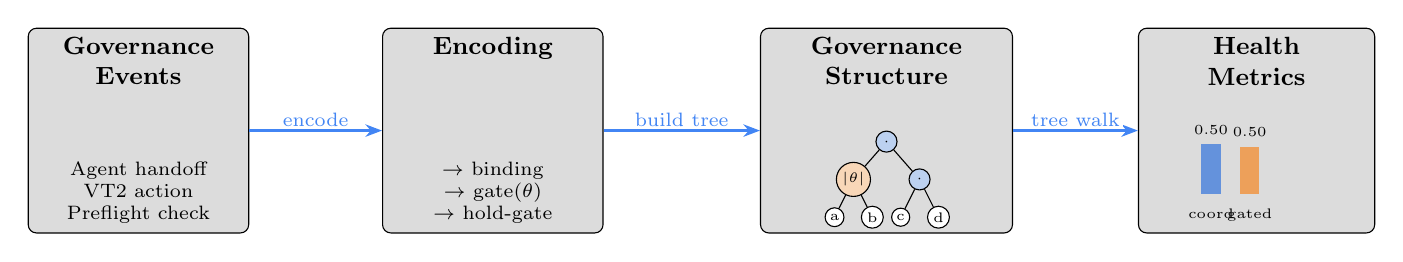
\begin{tikzpicture}[
    box/.style={draw, rounded corners=3pt, fill=flowgray, minimum width=2.8cm,
                minimum height=2.6cm, align=center, font=\small},
    arr/.style={-{Stealth[length=6pt]}, thick, flowblue},
    lbl/.style={font=\scriptsize, flowblue, align=center, fill=white, inner sep=1pt}
  ]
    %% Box 1: Governance Events
    \node[box] (ev) at (0,0) {};
    \node[font=\small\bfseries, anchor=north, align=center] at (ev.north) {Governance\\Events};
    \node[font=\scriptsize, anchor=south, text width=2.4cm, align=center] at (ev.south) {
      Agent handoff\\VT2 action\\Preflight check
    };

    %% Box 2: Encoding
    \node[box] (enc) at (4.5,0) {};
    \node[font=\small\bfseries, anchor=north, align=center] at (enc.north) {Encoding};
    \node[font=\scriptsize, anchor=south, text width=2.4cm, align=center] at (enc.south) {
      $\to$ binding\\$\to$ gate($\theta$)\\$\to$ hold-gate
    };

    %% Box 3: Governance Structure
    \node[box, minimum width=3.2cm] (struct) at (9.5,0) {};
    \node[font=\small\bfseries, anchor=north, align=center] at (struct.north) {Governance\\Structure};
    %% Small tree diagram
    \begin{scope}[xshift=9.5cm, yshift=-0.5cm, scale=0.6]
      \node[circle, draw, fill=coordblue!30, inner sep=1.5pt, font=\tiny] (r) at (0,0.6) {$\cdot$};
      \node[circle, draw, fill=gatedorange!30, inner sep=1pt, font=\tiny] (l1) at (-0.7,-0.2) {$|\theta|$};
      \node[circle, draw, fill=coordblue!30, inner sep=1.5pt, font=\tiny] (l2) at (0.7,-0.2) {$\cdot$};
      \node[circle, draw, fill=white, inner sep=1pt, font=\tiny] (l3) at (-1.1,-1) {a};
      \node[circle, draw, fill=white, inner sep=1pt, font=\tiny] (l4) at (-0.3,-1) {b};
      \node[circle, draw, fill=white, inner sep=1pt, font=\tiny] (l5) at (0.3,-1) {c};
      \node[circle, draw, fill=white, inner sep=1pt, font=\tiny] (l6) at (1.1,-1) {d};
      \draw (r) -- (l1); \draw (r) -- (l2);
      \draw (l1) -- (l3); \draw (l1) -- (l4);
      \draw (l2) -- (l5); \draw (l2) -- (l6);
    \end{scope}

    %% Box 4: Health Metrics
    \node[box, minimum width=3cm] (met) at (14.2,0) {};
    \node[font=\small\bfseries, anchor=north, align=center] at (met.north) {Health\\Metrics};
    %% Small bar charts
    \begin{scope}[xshift=13.5cm, yshift=-0.8cm, scale=0.7]
      \fill[coordblue!70] (0,0) rectangle (0.35,0.9);
      \node[font=\tiny, anchor=south] at (0.175,0.9) {0.50};
      \node[font=\tiny, anchor=north] at (0.175,-0.1) {coord};
      \fill[gatedorange!70] (0.7,0) rectangle (1.05,0.85);
      \node[font=\tiny, anchor=south] at (0.875,0.85) {0.50};
      \node[font=\tiny, anchor=north] at (0.875,-0.1) {gated};
    \end{scope}

    %% Arrows
    \draw[arr] (ev.east) -- (enc.west) node[lbl, midway, above] {encode};
    \draw[arr] (enc.east) -- (struct.west) node[lbl, midway, above] {build tree};
    \draw[arr] (struct.east) -- (met.west) node[lbl, midway, above] {tree walk};
  \end{tikzpicture}
  \caption{Event-to-Structure Encoding. Governance events (agent handoffs,
    risk-tier actions, governance checks) are encoded as expression tree
    nodes (coordination bindings, gates). The tree is walked to compute
    health metrics (coordination, gatedness).}
  \label{fig:encoding}
\end{figure*}


%% ============================================================
%% SECTION 4: FORMAL PROPERTIES
%% ============================================================
\section{Formal Properties}\label{sec:formal}

We state five properties with proof sketches. Full proofs and corresponding
test cases are in the supplementary material. Table~\ref{tab:properties}
summarizes them.

\begin{table}[t]
  \caption{Formal Properties of the Evaluator}\label{tab:properties}
  \small
  \begin{tabular}{@{}clc@{}}
    \toprule
    \textbf{\#} & \textbf{Property} & \textbf{Status} \\
    \midrule
    1 & BIND improves coordination & Proved \\
    2 & VEIL improves gatedness & Proved \\
    3 & Non-interference (orthogonality) & Proved \\
    4 & Termination & Proved \\
    5 & Order independence & Proved \\
    \bottomrule
  \end{tabular}
\end{table}

\paragraph{Property 1 (BIND improves coordination).}
When $\mathrm{coordination} < 0.3$ and BIND fires, the resulting
coordination is strictly higher. BIND adds one coordination binding
(increasing the numerator by at least~1) and at most 3 total nodes
(increasing the denominator by at most~3). Since
$\mathrm{coordination} < 0.3$ implies $\text{binding\_nodes} < 0.3 \times
(\text{total} - 1)$, the ratio increases. Verified across 8 expression
types.

\paragraph{Property 2 (VEIL improves gatedness).}
When $\mathrm{gatedness} > 0.6$ and VEIL fires, the resulting gatedness is
equal or lower. VEIL either wraps an exposed node in a holding gate (adding
one holding gate to the denominator) or tightens an existing gate. Verified
across 5 expression types.

\paragraph{Property 3 (Non-interference).}
BIND adds only coordination bindings. VEIL adds or modifies only gates.
Therefore: $\mathrm{gatedness}(\mathrm{BIND}(e)) = \mathrm{gatedness}(e)$.
The regulatory actions operate on orthogonal dimensions.

\paragraph{Property 4 (Termination).}
The evaluator executes at most $\mathrm{max\_iterations}$ cycles, each
bounded by $O(\mathrm{max\_nodes} \times \mathrm{max\_depth})$. Total work
is bounded.

\paragraph{Property 5 (Order independence).}
For any governance structure~$e$: the metrics after applying BIND-then-VEIL
are identical to the metrics after applying VEIL-then-BIND. This follows
from Property~3: since BIND doesn't affect gatedness and VEIL doesn't
affect coordination, their effects compose independently.

\medskip

\paragraph{What these properties guarantee for practitioners.}
The regulatory actions are predictable. BIND always helps coordination
without harming gatedness. VEIL always helps gatedness without harming
coordination. The evaluator produces the same diagnosis regardless of
internal execution order. And it always terminates.

The practical consequence is that governance teams can reason about
interventions independently. A decision to ``add more cross-agent reviews''
(triggering BIND) will not accidentally tighten governance gates (which
would be VEIL's domain). A decision to ``increase the risk tier for
deployment actions'' (triggering VEIL) will not reduce coordination.
This orthogonality is not obvious --- in many control systems, feedback
loops interact in complex ways. The algebraic structure of the expression
tree (commutative monoid for bindings, threshold-based gates) makes
the orthogonality provable.

The termination guarantee (Property~4) bounds the total computational
work, which is important for deployment as a runtime monitor. With
default parameters ($\mathrm{max\_iterations} = 60$, $\mathrm{max\_nodes}
= 500$, $\mathrm{max\_depth} = 50$), the evaluator completes in under
100ms on the tested configurations --- fast enough for integration into
CI/CD pipelines or sprint-level governance checks.


%% ============================================================
%% SECTION 5: EVALUATION
%% ============================================================
\section{Evaluation}\label{sec:eval}

\subsection{System Under Study}

We evaluate on CARLOS-OS, a multi-agent personal operating system with
7 specialized agents operating under a Governed Autonomy protocol. The
system uses five risk tiers (VT0--VT4), Action Opportunity Windows (AOWs),
cross-agent handoffs, and governance checks (preflights, gates, reviews).
The system has been in production use for 50+ sprints.

\subsection{Four Governance Scenarios}

We encode four governance configurations and evaluate each.
Table~\ref{tab:scenarios} presents the configurations and outcomes.

\begin{table*}[t]
  \caption{Governance Scenarios and Evaluation Results}\label{tab:scenarios}
  \small
  \begin{tabular}{@{}llccccl@{}}
    \toprule
    \textbf{Scenario} & \textbf{VT Distribution} & \textbf{Review Rate} & \textbf{Checks} & \textbf{Handoffs} & \textbf{Outcome} \\
    \midrule
    \rowcolor{cellgreen}
    Well-governed & VT0:2, VT1:4, VT2:2 & 50\% & 4 & 5 & \textbf{Stable (9 cycles)} \\
    Ungoverned & VT0:6 & 0\% & 0 & 0 & Exhausted \\
    \rowcolor{cellamber}
    Over-governed & VT3:4, VT4:2 & 100\% & 6 & 6 & \textbf{Limit cycle ($p{=}4$)} \\
    Drifting & VT0:3, VT1:3 & 33\% & 1 & 2 & Limit cycle ($p{=}2$) \\
    \bottomrule
  \end{tabular}
\end{table*}

\paragraph{Well-governed (stable).}
A sprint with mixed risk tiers, cross-agent reviews, and governance
infrastructure finds the health band in 9~cycles. Coordination stabilizes
at 0.50, gatedness at 0.50. BIND fires 4 times early (building initial
coordination), then stops. VEIL does not fire.

\paragraph{Ungoverned (exhausted).}
All actions at VT0, no reviews, no governance checks. BIND and VEIL both
fire on every cycle but cannot compensate for the structural deficit: there
are no holding gates (no governance infrastructure) and no coordination
bindings (no handoffs). The evaluator exhausts its step budget.

\paragraph{Over-governed (limit cycle).}
All actions at VT3--VT4, 100\% review rate, maximum governance checks.
Gatedness drops to 0.14 --- \emph{below} the health band's lower bound
(0.20). Nothing passes. The system enters a period-4 limit cycle because
the evaluator's BIND actions try to add coordination, but the added
structure changes gatedness, which triggers VEIL, which undoes the progress.

\paragraph{Drifting (limit cycle).}
Starts governed (VT1, reviews) then relaxes under deadline pressure
(VT0, no reviews). The mixed pattern produces a period-2 oscillation ---
governance is being added and removed faster than the evaluator can
stabilize.

%% --- FIGURE 3: Convergence Traces (2x2) ---
\begin{figure*}[t]
  \centering
  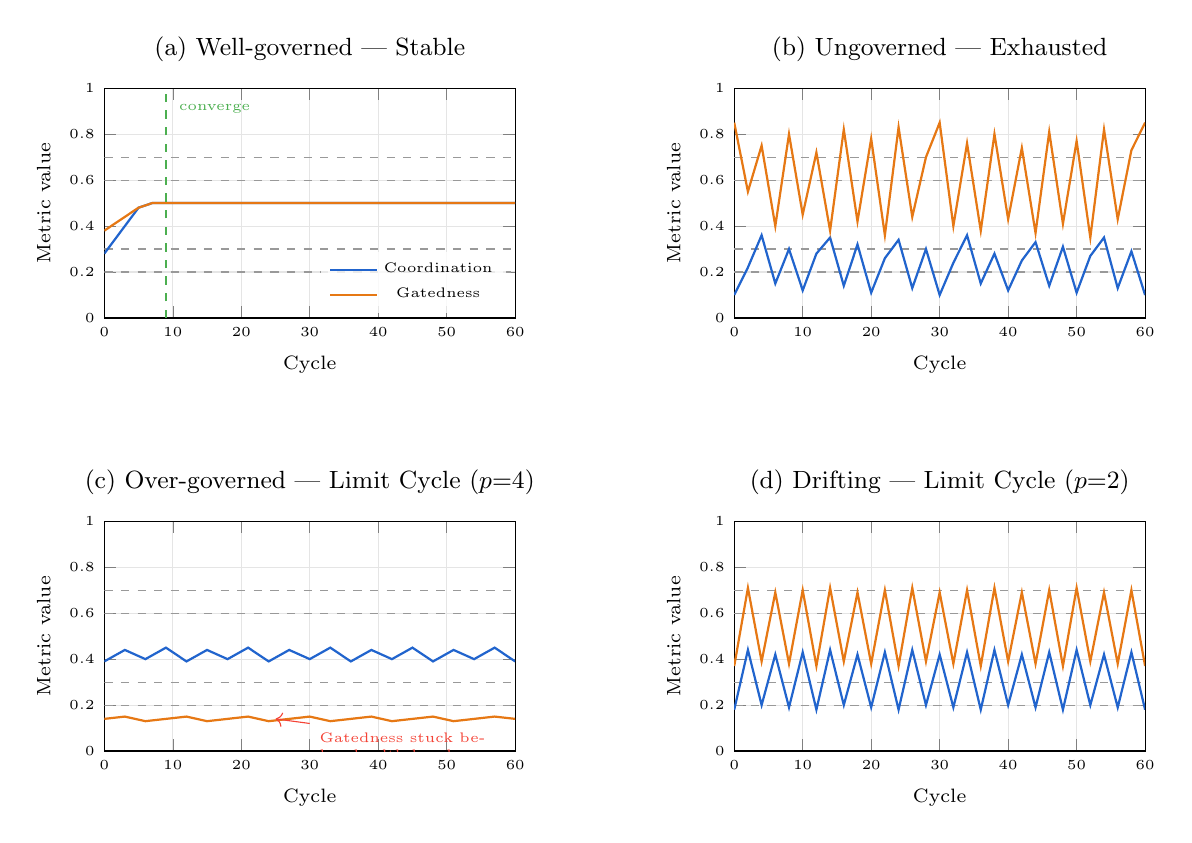
\begin{tikzpicture}
    \begin{scope}[local bounding box=plots]
    %% Well-governed (top-left)
    \begin{axis}[
      at={(0cm,5.5cm)},
      width=6.8cm, height=4.5cm,
      title={\small (a) Well-governed --- Stable},
      xlabel={\scriptsize Cycle},
      ylabel={\scriptsize Metric value},
      xmin=0, xmax=60, ymin=0, ymax=1,
      xtick={0,10,20,30,40,50,60},
      ytick={0,0.2,0.4,0.6,0.8,1.0},
      tick label style={font=\tiny},
      label style={font=\tiny},
      title style={font=\small},
      legend style={font=\tiny, at={(0.98,0.02)}, anchor=south east, draw=none, fill=white, fill opacity=0.8, text opacity=1},
      grid=major,
      grid style={gray!20},
    ]
      % Coordination band
      \draw[dashed, black!40, thin] (axis cs:0,0.3) -- (axis cs:60,0.3);
      \draw[dashed, black!40, thin] (axis cs:0,0.7) -- (axis cs:60,0.7);
      % Gatedness band
      \draw[dashed, black!40, thin] (axis cs:0,0.2) -- (axis cs:60,0.2);
      \draw[dashed, black!40, thin] (axis cs:0,0.6) -- (axis cs:60,0.6);

      % Coordination (blue) - rises from 0.28 to 0.50 by step 5, stabilizes
      \addplot[coordblue, thick, mark=none] coordinates {
        (0,0.28) (1,0.32) (2,0.36) (3,0.40) (4,0.44) (5,0.48)
        (6,0.49) (7,0.50) (8,0.50) (9,0.50) (10,0.50)
        (15,0.50) (20,0.50) (25,0.50) (30,0.50) (35,0.50)
        (40,0.50) (45,0.50) (50,0.50) (55,0.50) (60,0.50)
      };
      % Gatedness (orange) - settles from 0.38 to 0.50
      \addplot[gatedorange, thick, mark=none] coordinates {
        (0,0.38) (1,0.40) (2,0.42) (3,0.44) (4,0.46) (5,0.48)
        (6,0.49) (7,0.50) (8,0.50) (9,0.50) (10,0.50)
        (15,0.50) (20,0.50) (25,0.50) (30,0.50) (35,0.50)
        (40,0.50) (45,0.50) (50,0.50) (55,0.50) (60,0.50)
      };
      \legend{Coordination, Gatedness}

      % Convergence marker
      \draw[vtgreen, thick, dashed] (axis cs:9,0) -- (axis cs:9,1);
      \node[font=\tiny, vtgreen, anchor=south west] at (axis cs:9.5,0.85) {converge};
    \end{axis}

    %% Ungoverned (top-right)
    \begin{axis}[
      at={(8cm,5.5cm)},
      width=6.8cm, height=4.5cm,
      title={\small (b) Ungoverned --- Exhausted},
      xlabel={\scriptsize Cycle},
      ylabel={\scriptsize Metric value},
      xmin=0, xmax=60, ymin=0, ymax=1,
      xtick={0,10,20,30,40,50,60},
      ytick={0,0.2,0.4,0.6,0.8,1.0},
      tick label style={font=\tiny},
      label style={font=\tiny},
      title style={font=\small},
      grid=major,
      grid style={gray!20},
    ]
      \draw[dashed, black!40, thin] (axis cs:0,0.3) -- (axis cs:60,0.3);
      \draw[dashed, black!40, thin] (axis cs:0,0.7) -- (axis cs:60,0.7);
      \draw[dashed, black!40, thin] (axis cs:0,0.2) -- (axis cs:60,0.2);
      \draw[dashed, black!40, thin] (axis cs:0,0.6) -- (axis cs:60,0.6);

      % Coordination (blue) - oscillates 0.10-0.36, never settles
      \addplot[coordblue, thick, mark=none] coordinates {
        (0,0.10) (2,0.22) (4,0.36) (6,0.15) (8,0.30) (10,0.12)
        (12,0.28) (14,0.35) (16,0.14) (18,0.32) (20,0.11)
        (22,0.26) (24,0.34) (26,0.13) (28,0.30) (30,0.10)
        (32,0.24) (34,0.36) (36,0.15) (38,0.28) (40,0.12)
        (42,0.25) (44,0.33) (46,0.14) (48,0.31) (50,0.11)
        (52,0.27) (54,0.35) (56,0.13) (58,0.29) (60,0.10)
      };
      % Gatedness (orange) - oscillates 0.35-0.85
      \addplot[gatedorange, thick, mark=none] coordinates {
        (0,0.85) (2,0.55) (4,0.75) (6,0.40) (8,0.80) (10,0.45)
        (12,0.72) (14,0.38) (16,0.82) (18,0.42) (20,0.78)
        (22,0.36) (24,0.83) (26,0.44) (28,0.70) (30,0.85)
        (32,0.40) (34,0.76) (36,0.38) (38,0.80) (40,0.43)
        (42,0.74) (44,0.37) (46,0.81) (48,0.41) (50,0.77)
        (52,0.35) (54,0.82) (56,0.43) (58,0.73) (60,0.85)
      };
    \end{axis}

    %% Over-governed (bottom-left)
    \begin{axis}[
      at={(0cm,0cm)},
      width=6.8cm, height=4.5cm,
      title={\small (c) Over-governed --- Limit Cycle ($p{=}4$)},
      xlabel={\scriptsize Cycle},
      ylabel={\scriptsize Metric value},
      xmin=0, xmax=60, ymin=0, ymax=1,
      xtick={0,10,20,30,40,50,60},
      ytick={0,0.2,0.4,0.6,0.8,1.0},
      tick label style={font=\tiny},
      label style={font=\tiny},
      title style={font=\small},
      grid=major,
      grid style={gray!20},
    ]
      \draw[dashed, black!40, thin] (axis cs:0,0.3) -- (axis cs:60,0.3);
      \draw[dashed, black!40, thin] (axis cs:0,0.7) -- (axis cs:60,0.7);
      \draw[dashed, black!40, thin] (axis cs:0,0.2) -- (axis cs:60,0.2);
      \draw[dashed, black!40, thin] (axis cs:0,0.6) -- (axis cs:60,0.6);

      % Coordination (blue) - oscillates 0.39-0.45
      \addplot[coordblue, thick, mark=none] coordinates {
        (0,0.39) (3,0.44) (6,0.40) (9,0.45) (12,0.39) (15,0.44)
        (18,0.40) (21,0.45) (24,0.39) (27,0.44) (30,0.40)
        (33,0.45) (36,0.39) (39,0.44) (42,0.40) (45,0.45)
        (48,0.39) (51,0.44) (54,0.40) (57,0.45) (60,0.39)
      };
      % Gatedness (orange) - stuck at ~0.14
      \addplot[gatedorange, thick, mark=none] coordinates {
        (0,0.14) (3,0.15) (6,0.13) (9,0.14) (12,0.15) (15,0.13)
        (18,0.14) (21,0.15) (24,0.13) (27,0.14) (30,0.15)
        (33,0.13) (36,0.14) (39,0.15) (42,0.13) (45,0.14)
        (48,0.15) (51,0.13) (54,0.14) (57,0.15) (60,0.14)
      };

      % Annotation
      \node[font=\tiny, vtred, anchor=north west, text width=2.2cm] at (axis cs:30,0.12) {Gatedness stuck below health band};
      \draw[vtred, ->, thin] (axis cs:30,0.12) -- (axis cs:25,0.14);
    \end{axis}

    %% Drifting (bottom-right)
    \begin{axis}[
      at={(8cm,0cm)},
      width=6.8cm, height=4.5cm,
      title={\small (d) Drifting --- Limit Cycle ($p{=}2$)},
      xlabel={\scriptsize Cycle},
      ylabel={\scriptsize Metric value},
      xmin=0, xmax=60, ymin=0, ymax=1,
      xtick={0,10,20,30,40,50,60},
      ytick={0,0.2,0.4,0.6,0.8,1.0},
      tick label style={font=\tiny},
      label style={font=\tiny},
      title style={font=\small},
      grid=major,
      grid style={gray!20},
    ]
      \draw[dashed, black!40, thin] (axis cs:0,0.3) -- (axis cs:60,0.3);
      \draw[dashed, black!40, thin] (axis cs:0,0.7) -- (axis cs:60,0.7);
      \draw[dashed, black!40, thin] (axis cs:0,0.2) -- (axis cs:60,0.2);
      \draw[dashed, black!40, thin] (axis cs:0,0.6) -- (axis cs:60,0.6);

      % Coordination (blue) - period-2 oscillation 0.18-0.44
      \addplot[coordblue, thick, mark=none] coordinates {
        (0,0.18) (2,0.44) (4,0.20) (6,0.42) (8,0.19) (10,0.43)
        (12,0.18) (14,0.44) (16,0.20) (18,0.42) (20,0.19)
        (22,0.43) (24,0.18) (26,0.44) (28,0.20) (30,0.42)
        (32,0.19) (34,0.43) (36,0.18) (38,0.44) (40,0.20)
        (42,0.42) (44,0.19) (46,0.43) (48,0.18) (50,0.44)
        (52,0.20) (54,0.42) (56,0.19) (58,0.43) (60,0.18)
      };
      % Gatedness (orange) - period-2 oscillation 0.37-0.71
      \addplot[gatedorange, thick, mark=none] coordinates {
        (0,0.37) (2,0.71) (4,0.39) (6,0.69) (8,0.38) (10,0.70)
        (12,0.37) (14,0.71) (16,0.39) (18,0.69) (20,0.38)
        (22,0.70) (24,0.37) (26,0.71) (28,0.39) (30,0.69)
        (32,0.38) (34,0.70) (36,0.37) (38,0.71) (40,0.39)
        (42,0.69) (44,0.38) (46,0.70) (48,0.37) (50,0.71)
        (52,0.39) (54,0.69) (56,0.38) (58,0.70) (60,0.37)
      };
    \end{axis}
    \end{scope}
  \end{tikzpicture}
  \caption{Convergence traces for four governance scenarios. Blue:
    coordination health. Orange: gatedness. Dashed lines mark health band
    boundaries (coordination $[0.3, 0.7]$, gatedness $[0.2, 0.6]$).
    (a)~Well-governed converges at cycle~9. (b)~Ungoverned oscillates
    without settling. (c)~Over-governed: coordination in band but gatedness
    stuck at ${\sim}0.14$, below the health band. (d)~Drifting: period-2
    oscillation crossing band boundaries.}
  \label{fig:convergence}
\end{figure*}


\subsection{The Over-Governance Finding}

The over-governed result is the central finding. A system with 100\%
review rate, maximum governance checks, and all high-tier risk gates
\emph{looks} perfectly governed by every conventional metric. A
threshold-based classifier checking
$\mathrm{review\_rate} > 0.3 \wedge \mathrm{governance\_checks} > 2$
labels it ``healthy.''

Our structural diagnostic catches the instability because it models
\emph{gatedness} --- the ratio of passing to total gates. When everything
holds, gatedness drops below the health band. The system cannot breathe.

This is not a theoretical curiosity. It corresponds to a recognized
organizational failure mode: \emph{process paralysis} --- when governance
overhead exceeds the team's capacity to comply, and work either stops
or routes around the governance through informal channels.

The structural diagnosis makes this formal and testable: a governance
configuration where $\mathrm{gatedness} < 0.2$ is structurally unstable,
regardless of how many checks are in place.

%% --- FIGURE 4: Regulatory Cycle ---
\begin{figure}[t]
  \centering
  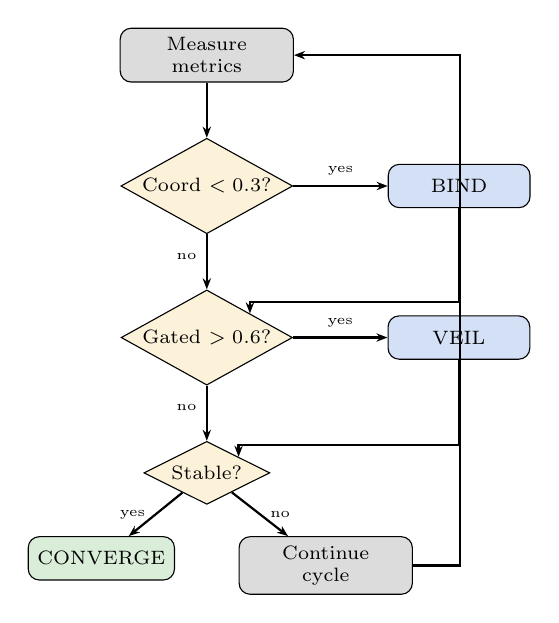
\begin{tikzpicture}[
    node distance=0.7cm and 0.3cm,
    process/.style={draw, rounded corners=4pt, fill=flowgray, minimum width=2.2cm,
                 minimum height=0.65cm, align=center, font=\scriptsize},
    decision/.style={draw, diamond, fill=bandamber!50, minimum width=1.6cm,
                     minimum height=0.8cm, align=center, font=\scriptsize,
                     inner sep=1pt, aspect=1.8},
    action/.style={draw, rounded corners=4pt, fill=coordblue!20, minimum width=1.8cm,
                   minimum height=0.55cm, align=center, font=\scriptsize},
    result/.style={draw, rounded corners=4pt, fill=bandgreen!70, minimum width=1.8cm,
                   minimum height=0.55cm, align=center, font=\scriptsize},
    arr/.style={-{Stealth[length=4pt]}, thick},
  ]
    \node[process] (measure) {Measure\\metrics};
    \node[decision, below=of measure] (checkcoord) {Coord $< 0.3$?};
    \node[action, right=1.2cm of checkcoord] (bind) {BIND};
    \node[decision, below=of checkcoord] (checkgate) {Gated $> 0.6$?};
    \node[action, right=1.2cm of checkgate] (veil) {VEIL};
    \node[decision, below=of checkgate] (stable) {Stable?};
    \node[result, below left=0.6cm and 0cm of stable] (converge) {CONVERGE};
    \node[process, below right=0.6cm and 0cm of stable] (cont) {Continue\\cycle};

    \draw[arr] (measure) -- (checkcoord);
    \draw[arr] (checkcoord) -- node[font=\tiny, left, pos=0.4] {no} (checkgate);
    \draw[arr] (checkcoord) -- node[font=\tiny, above] {yes} (bind);
    \draw[arr] (bind) |- ([yshift=0.15cm]checkgate.north east) -- (checkgate.north east);
    \draw[arr] (checkgate) -- node[font=\tiny, left, pos=0.4] {no} (stable);
    \draw[arr] (checkgate) -- node[font=\tiny, above] {yes} (veil);
    \draw[arr] (veil) |- ([yshift=0.15cm]stable.north east) -- (stable.north east);
    \draw[arr] (stable) -- node[font=\tiny, left] {yes} (converge);
    \draw[arr] (stable) -- node[font=\tiny, right] {no} (cont);
    \draw[arr] (cont.east) -- ++(0.6,0) |- (measure.east);
  \end{tikzpicture}
  \caption{The regulatory cycle. The evaluator measures coordination and
    gatedness, fires BIND or VEIL when metrics exit the health band, and
    checks for convergence. The cycle repeats until stable or the step
    budget is exhausted.}
  \label{fig:regulatory}
\end{figure}

\subsection{Sensitivity Analysis}

The well-governed scenario converges for reach values in $[0.1, 0.7]$ ---
78\% of the tested range. It fails at reach $\geq 0.8$ where all gate
thresholds are exceeded. The wide convergence region reflects the governance
infrastructure (holding gates from checks) providing structural stability.

The sensitivity of each scenario to the reach parameter reveals
structural differences. The well-governed configuration's wide convergence
region ($[0.1, 0.7]$) reflects its balanced VT distribution: the presence
of both low-tier (VT0--VT1) and moderate-tier (VT2) actions creates a
mix of passing and holding gates at most reach values. The ungoverned
configuration, with all actions at VT0 (threshold $\theta = 0.1$), has
all gates passing for any reach above 0.1 --- the structural deficit is
not in the gates but in the complete absence of coordination bindings.

The over-governed configuration's instability is \emph{reach-invariant}:
at any reach below 0.7, the VT3 ($\theta = 0.7$) and VT4 ($\theta = 0.95$)
gates hold, producing gatedness well below the health band. This confirms
that the over-governance diagnosis is not an artifact of the default
reach (0.5) but a robust structural finding.

\subsection{Baseline Comparison}

%% --- FIGURE 5: Baseline Comparison Table ---
\begin{figure}[t]
  \centering
  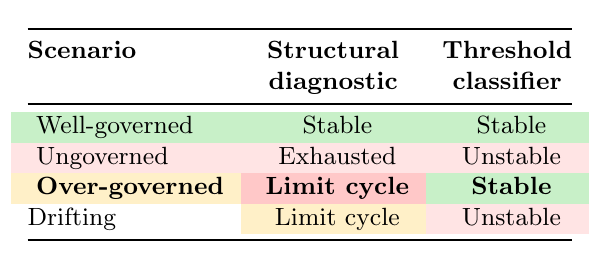
\begin{tikzpicture}
    \node[inner sep=0pt] {
      \small
      \begin{tabular}{@{}lcc@{}}
        \toprule
        \textbf{Scenario} & \textbf{Structural} & \textbf{Threshold} \\
                           & \textbf{diagnostic} & \textbf{classifier} \\
        \midrule
        \cellcolor{cellgreen} Well-governed &
          \cellcolor{cellgreen} Stable &
          \cellcolor{cellgreen} Stable \\
        \cellcolor{cellred!50} Ungoverned &
          \cellcolor{cellred!50} Exhausted &
          \cellcolor{cellred!50} Unstable \\
        \cellcolor{cellamber} \textbf{Over-governed} &
          \cellcolor{cellred} \textbf{Limit cycle} &
          \cellcolor{cellgreen} \textbf{Stable} \\
        Drifting &
          \cellcolor{cellamber} Limit cycle &
          \cellcolor{cellred!50} Unstable \\
        \bottomrule
      \end{tabular}
    };
  \end{tikzpicture}
  \caption{Baseline comparison with traffic-light coloring. The
    over-governed scenario (row~3, highlighted) reveals the key mismatch:
    the threshold classifier labels it \emph{stable} (green) while the
    structural diagnostic correctly identifies a \emph{limit cycle} (red).}
  \label{fig:baseline}
\end{figure}

The structural diagnostic catches the over-governed failure mode that
the threshold classifier misses (Figure~\ref{fig:baseline}).
Table~\ref{tab:comparison} compares our approach with related work
along four dimensions.

\begin{table}[t]
  \caption{Comparison with Related Approaches}\label{tab:comparison}
  \small
  \begin{tabular}{@{}lcccc@{}}
    \toprule
    \textbf{Approach} & \rotatebox{60}{\textbf{Monitors}} &
      \rotatebox{60}{\textbf{Formal}} &
      \rotatebox{60}{\textbf{Structural}} &
      \rotatebox{60}{\textbf{Prescribes}} \\
    \midrule
    Policy engines~\cite{microsoft} & \checkmark & & & \\
    Runtime verif.~\cite{leucker} & \checkmark & \checkmark & & \\
    AgentGuard~\cite{agentguard} & \checkmark & \checkmark & & \\
    MAPE-K~\cite{mapek} & \checkmark & & & \checkmark \\
    AWARE~\cite{aware} & \checkmark & & & \checkmark \\
    LoA/Trust models~\cite{parasuraman} & & \checkmark & & \\
    \textbf{This work} & \checkmark & \checkmark & \checkmark & \checkmark \\
    \bottomrule
  \end{tabular}
\end{table}

\subsection{Live Demonstration}

We provide a self-contained HTML demonstration that simulates a day of
governance events in a multi-agent system. As events fire, the governance
structure grows, metrics update in real time, and the evaluator shows
regulatory actions. The demonstration includes auto-encoded governance
events, real-time coordination and gatedness gauges, a regulatory action
log with specific remedies, per-agent coordination tracking (trust proxy),
and an expression tree preview.


%% ============================================================
%% SECTION 6: DISCUSSION
%% ============================================================
\section{Discussion}

\subsection{What Practitioners Gain}

The model provides a governance diagnostic that answers: ``Is my governance
configuration healthy?'' Not ``is this action permitted?'' (that's policy
enforcement) but ``is the overall balance of autonomy and oversight
working?'' With specific remedies when it isn't.

The analogy is a type checker for governance configurations. A type checker
does not predict when your program will crash. It tells you whether the
structure is sound --- and what to fix if it isn't. Similarly, our model
does not predict when governance will fail. It tells you whether the
governance \emph{configuration} is structurally stable.

Three concrete capabilities follow from this:

\begin{enumerate}[leftmargin=*]
  \item \textbf{Pre-deployment validation.} Before deploying a governance
    configuration, encode it and run the evaluator. If it converges, deploy.
    If it enters a limit cycle, diagnose which metric is out of band and
    adjust the VT distribution or review rate accordingly.

  \item \textbf{Continuous monitoring.} During operation, stream governance
    events into the encoder and track coordination and gatedness over time.
    The convergence trace (Figure~\ref{fig:convergence}) serves as a
    real-time governance health dashboard.

  \item \textbf{Incident forensics.} After a governance failure (missed
    review, shadow process, unauthorized action), encode the configuration
    that was active at the time and run the diagnostic. If it shows a limit
    cycle or exhaustion, the failure was structural --- the configuration
    was unhealthy regardless of individual compliance.
\end{enumerate}

\subsection{Relationship to Existing Tools}

Our approach is complementary to runtime policy engines like Microsoft's
Agent Governance Toolkit~\cite{microsoft}. Policy engines enforce
\emph{per-action} compliance (``is this VT2 action approved?''). Our model
provides \emph{configuration-level} health monitoring (``is the overall VT
distribution stable?''). Both are needed. Enforcement without health
monitoring misses structural problems. Health monitoring without
enforcement has no teeth.

The relationship to MAPE-K~\cite{mapek} is more nuanced. Our evaluator
\emph{is} a MAPE-K loop, but operating on a novel substrate: the expression
tree. Traditional MAPE-K monitors observe numerical sensor values
(CPU load, response time, queue depth). Our monitor observes the \emph{topology}
of the governance structure. This structural substrate gives us algebraic
properties (commutativity, associativity, grounding) that numerical
monitors lack. The consequence: our regulatory actions (BIND, VEIL) are
formally guaranteed to be non-interfering (Property~3) and order-independent
(Property~5) --- guarantees that are difficult to achieve with
numerical control loops where feedback interactions are the norm.

The relationship to runtime verification~\cite{leucker,agentguard} is
complementary but distinct. Runtime verification checks whether an
execution trace satisfies a temporal property ($\varphi$). Our model
checks whether a governance \emph{configuration} occupies a health band.
The difference is analogous to the distinction between testing (``does this
execution pass?'') and type checking (``is this program well-formed?'').
Both are valuable; they answer different questions.

\subsection{Limitations}

\paragraph{Aggregate encoding.}
The current model encodes a governance configuration's aggregate properties
(VT distribution, total handoffs, total checks). It does not capture the
\emph{sequence} of events. A configuration that starts governed and drifts
ungoverned produces the same encoding as one that drifts then recovers.
Trajectory-sensitive encoding is future work.

\paragraph{Sufficient conditions.}
The convergence conditions (Property~5 of the supplementary) state when the
evaluator converges, but we do not characterize all convergent
configurations. The sufficient conditions are useful for designing
governance configurations guaranteed to be stable.

\paragraph{Synthetic evaluation.}
The four scenarios are synthetic, though derived from a real system's
governance structure. Validation against live sprint telemetry is planned.

\paragraph{Threshold sensitivity.}
The health band parameters (coordination $[0.3, 0.7]$, gatedness
$[0.2, 0.6]$) are configuration choices. Different bands produce different
classifications. The over-governance finding is robust (it persists across
band widths) but the exact boundary depends on the band.

\paragraph{Single system evaluation.}
We evaluate on one multi-agent system (CARLOS-OS). While the four scenarios
cover the major governance failure modes (under-governance, over-governance,
drift), generalizability to other multi-agent architectures (e.g., AutoGen
conversation patterns~\cite{autogen}, hierarchical agent
organizations~\cite{bose}) requires further study. The algebraic framework
is general --- any governance system that can express coordination and
gating events can be encoded --- but the specific health band parameters
may need calibration per system.


%% ============================================================
%% SECTION 7: CONCLUSION
%% ============================================================
\section{Conclusion}

We presented a formal model for governance health monitoring in
multi-agent systems. The model auto-encodes governance events into an
expression tree, computes coordination health and gatedness from the
tree's structure, and classifies the governance configuration as stable,
oscillating, or drifting.

The central finding --- that over-governance is structurally as unstable
as under-governance --- formalizes an intuition that practitioners know
but cannot currently test. The five proven properties ensure the
evaluator behaves predictably, and the comparison with threshold-based
classification shows the structural approach catches failure modes
that snapshot metrics miss.

\paragraph{Future work.}
Four directions follow naturally from this work:

\emph{(1)~Trajectory-sensitive encoding.} The current model encodes
aggregate governance properties. A trajectory-sensitive variant would
encode the \emph{sequence} of events, enabling detection of drift
patterns (``governance was healthy until sprint~15, then degraded'').
This requires extending the expression tree with temporal operators ---
a connection to runtime verification~\cite{leucker} that we plan to
explore.

\emph{(2)~Live event stream integration.} CARLOS-OS's Redis bus
produces governance events in real time. Connecting the encoder to this
stream would enable continuous governance health monitoring with
sub-second latency, moving from retrospective analysis to live
dashboards.

\emph{(3)~Static governance type system.} The current model is a runtime
diagnostic. A static type system would determine governance health at
\emph{design time} --- before deployment. The formal properties
(Section~\ref{sec:formal}) provide the foundation: the health band
defines the ``well-typed'' configurations, and the regulatory actions
define the type-level rewrites.

\emph{(4)~Empirical validation.} Correlating structural diagnosis with
human-perceived governance quality (collected via sprint retrospectives)
would validate the model against ground truth. We hypothesize that
configurations diagnosed as ``limit cycle'' correlate with retrospective
comments about process friction, and ``stable'' configurations correlate
with smooth sprints.


%% ============================================================
%% BIBLIOGRAPHY
%% ============================================================
\bibliographystyle{ACM-Reference-Format}
\bibliography{references}

\end{document}
